\setcounter{page}{1}
\setcounter{figure}{0}  % reset counter

\section{Synthetic Phosphorylation Results}
\subsection{High Scoring Decoy Results}\label{sec:highScoringDecoyCharge3}
In order to validate the FLR approach, we used spectra from synthetic peptides aquired on an LTQ-Orbitrap XL CID.~\cite{savitski11} Full scan MS spectra were acquired in the Orbitrap at a resolution of $60,000$ at m/z $400$ after accumulating ions to a target value of $1*106$. The five most intense ions were selected for fragmentation by CID with a resolution of $.5$ Da for fragment tolerance . These $7,992$ CID spectra were then searched using \inspect ~\cite{tanner05} with $2$Da parent and $.5$ fragment tolerance against the $153$ proteins from which the $180$ peptides were synthesized plus $8$ common contaminant proteins at a cutoff of $1\%$ FDR. $966$ charge 2 spectra and $281$ charge 3 spectra were identified.

After performing our scoring For charge 3 data, as shown in Table~\ref{tbl:incorrectAssignments} there were a number of repeated incorrect hits from the same plate and well number (plate 1, well 11). According to the synthesis information, this should be LQ(T,80)VHSIPLTINK, but we identify as LQTVH(S,80)IPLTINK. There are a few possibilities that may account for this. The most likely case is that our unmodified spectrum does not closely resemble the fragmentation present in the modified spectrum. In this particular case, while there is a NIST spectrum of the same peptide, the cosine was not very high, so the MassAnalyzer prediction was used. The other possibility is that there may have been well crossover. In  plate 1 well B2, the modification peptide we identify is present. These two peptides are from different mixtures, however it is possible that since these are from the same synthesis plate, there was well crossover or another issue with contaminuation.

From manual inspection of the spectra both modification positions seem plausible (See  Figure~\ref{fig:charge3Incorrect}), though the identification of doubly charged y9 and y10 modified fragments seems to push the identification in the direction of our LQTVH(S,80)IPLTINK assignment. Likewise, there is a possible phosphorylated b5 ion (which we do not use in our scoring scheme) that indicates that LQ(T,80)VHSIPLTINK might be present.

\begin{table}[h]
\centering
\caption{Incorrect assignments at $1\%$ FLR}\label{tbl:incorrectAssignments}
\resizebox{7in}{!} {
\begin{tabular}{|l|l|l|l|l|l|l|l|}
File & Index & LP quantity & LP valid variants & Synthesis sequence & mixture & Synthesis plate & Synthesis Plate Position \\
\hline
ppeptidemix1\_CID\_Orbi.mgf & 981 & LQTVH(S,-18.0106)IPLTINK & LQ(T,-18.0106)VHSIPLTINK & 1 & Pep0001 & A11 \\
ppeptidemix1\_CID\_Orbi.mgf & 979 & LQTVH(S,-18.0106)IPLTINK & LQ(T,-18.0106)VHSIPLTINK & 1 & Pep0001 & A11 \\
ppeptidemix1\_CID\_Orbi.mgf & 996 & LQTVH(S,-18.0106)IPLTINK & LQ(T,-18.0106)VHSIPLTINK & 1 & Pep0001 & A11 \\
ppeptidemix1\_CID\_Orbi.mgf & 991 & LQTVH(S,-18.0106)IPLTINK & LQ(T,-18.0106)VHSIPLTINK & 1 & Pep0001 & A11 \\
ppeptidemix1\_CID\_Orbi.mgf & 975 & LQTVH(S,-18.0106)IPLTINK & LQ(T,-18.0106)VHSIPLTINK & 1 & Pep0001 & A11 \\
ppeptidemix1\_CID\_Orbi.mgf & 1005 & LQTVH(S,-18.0106)IPLTINK & LQ(T,-18.0106)VHSIPLTINK & 1 & Pep0001 & A11 \\
ppeptidemix3\_CID\_Orbi.mgf & 352 & AGIH(T,-18.0106)SGSLSSR & AGIHT(S,-18.0106)GSLSSR & 3 & Pep0002 & A11 \\
ppeptidemix5\_CID\_Orbi.mgf & 337 & ETTT(S,-18.0106)PKKYYLAEK & ET(T,-18.0106)TSPKKYYLAEK & 5 & Pep0008 & A9 \\
ppeptidemix4\_CID\_Orbi.mgf & 530 & ETTT(S,-18.0106)PKKYYLAEK & E(T,-18.0106)TTSPKKYYLAEK & 4 & Pep0008 & A8 \\
ppeptidemix1\_CID\_Orbi.mgf & 441 & ETTT(S,-18.0106)PKKYYLAEK & ETT(T,-18.0106)SPKKYYLAEK & 1 & Pep0008 & A10 \\
ppeptidemix5\_CID\_Orbi.mgf & 354 & ETTT(S,-18.0106)PKKYYLAEK & ET(T,-18.0106)TSPKKYYLAEK & 5 & Pep0008 & A9 \\
\hline
\end{tabular}
}
\end{table}

As shown in Figure~\ref{fig:charge3Incorrect}, this is primarily due to the fact that the doubly charged y6 fragment is not present in the unmodified spectra and therefore is labeled as a b3 ion.

\begin{figure}[h!]
\centering
a) 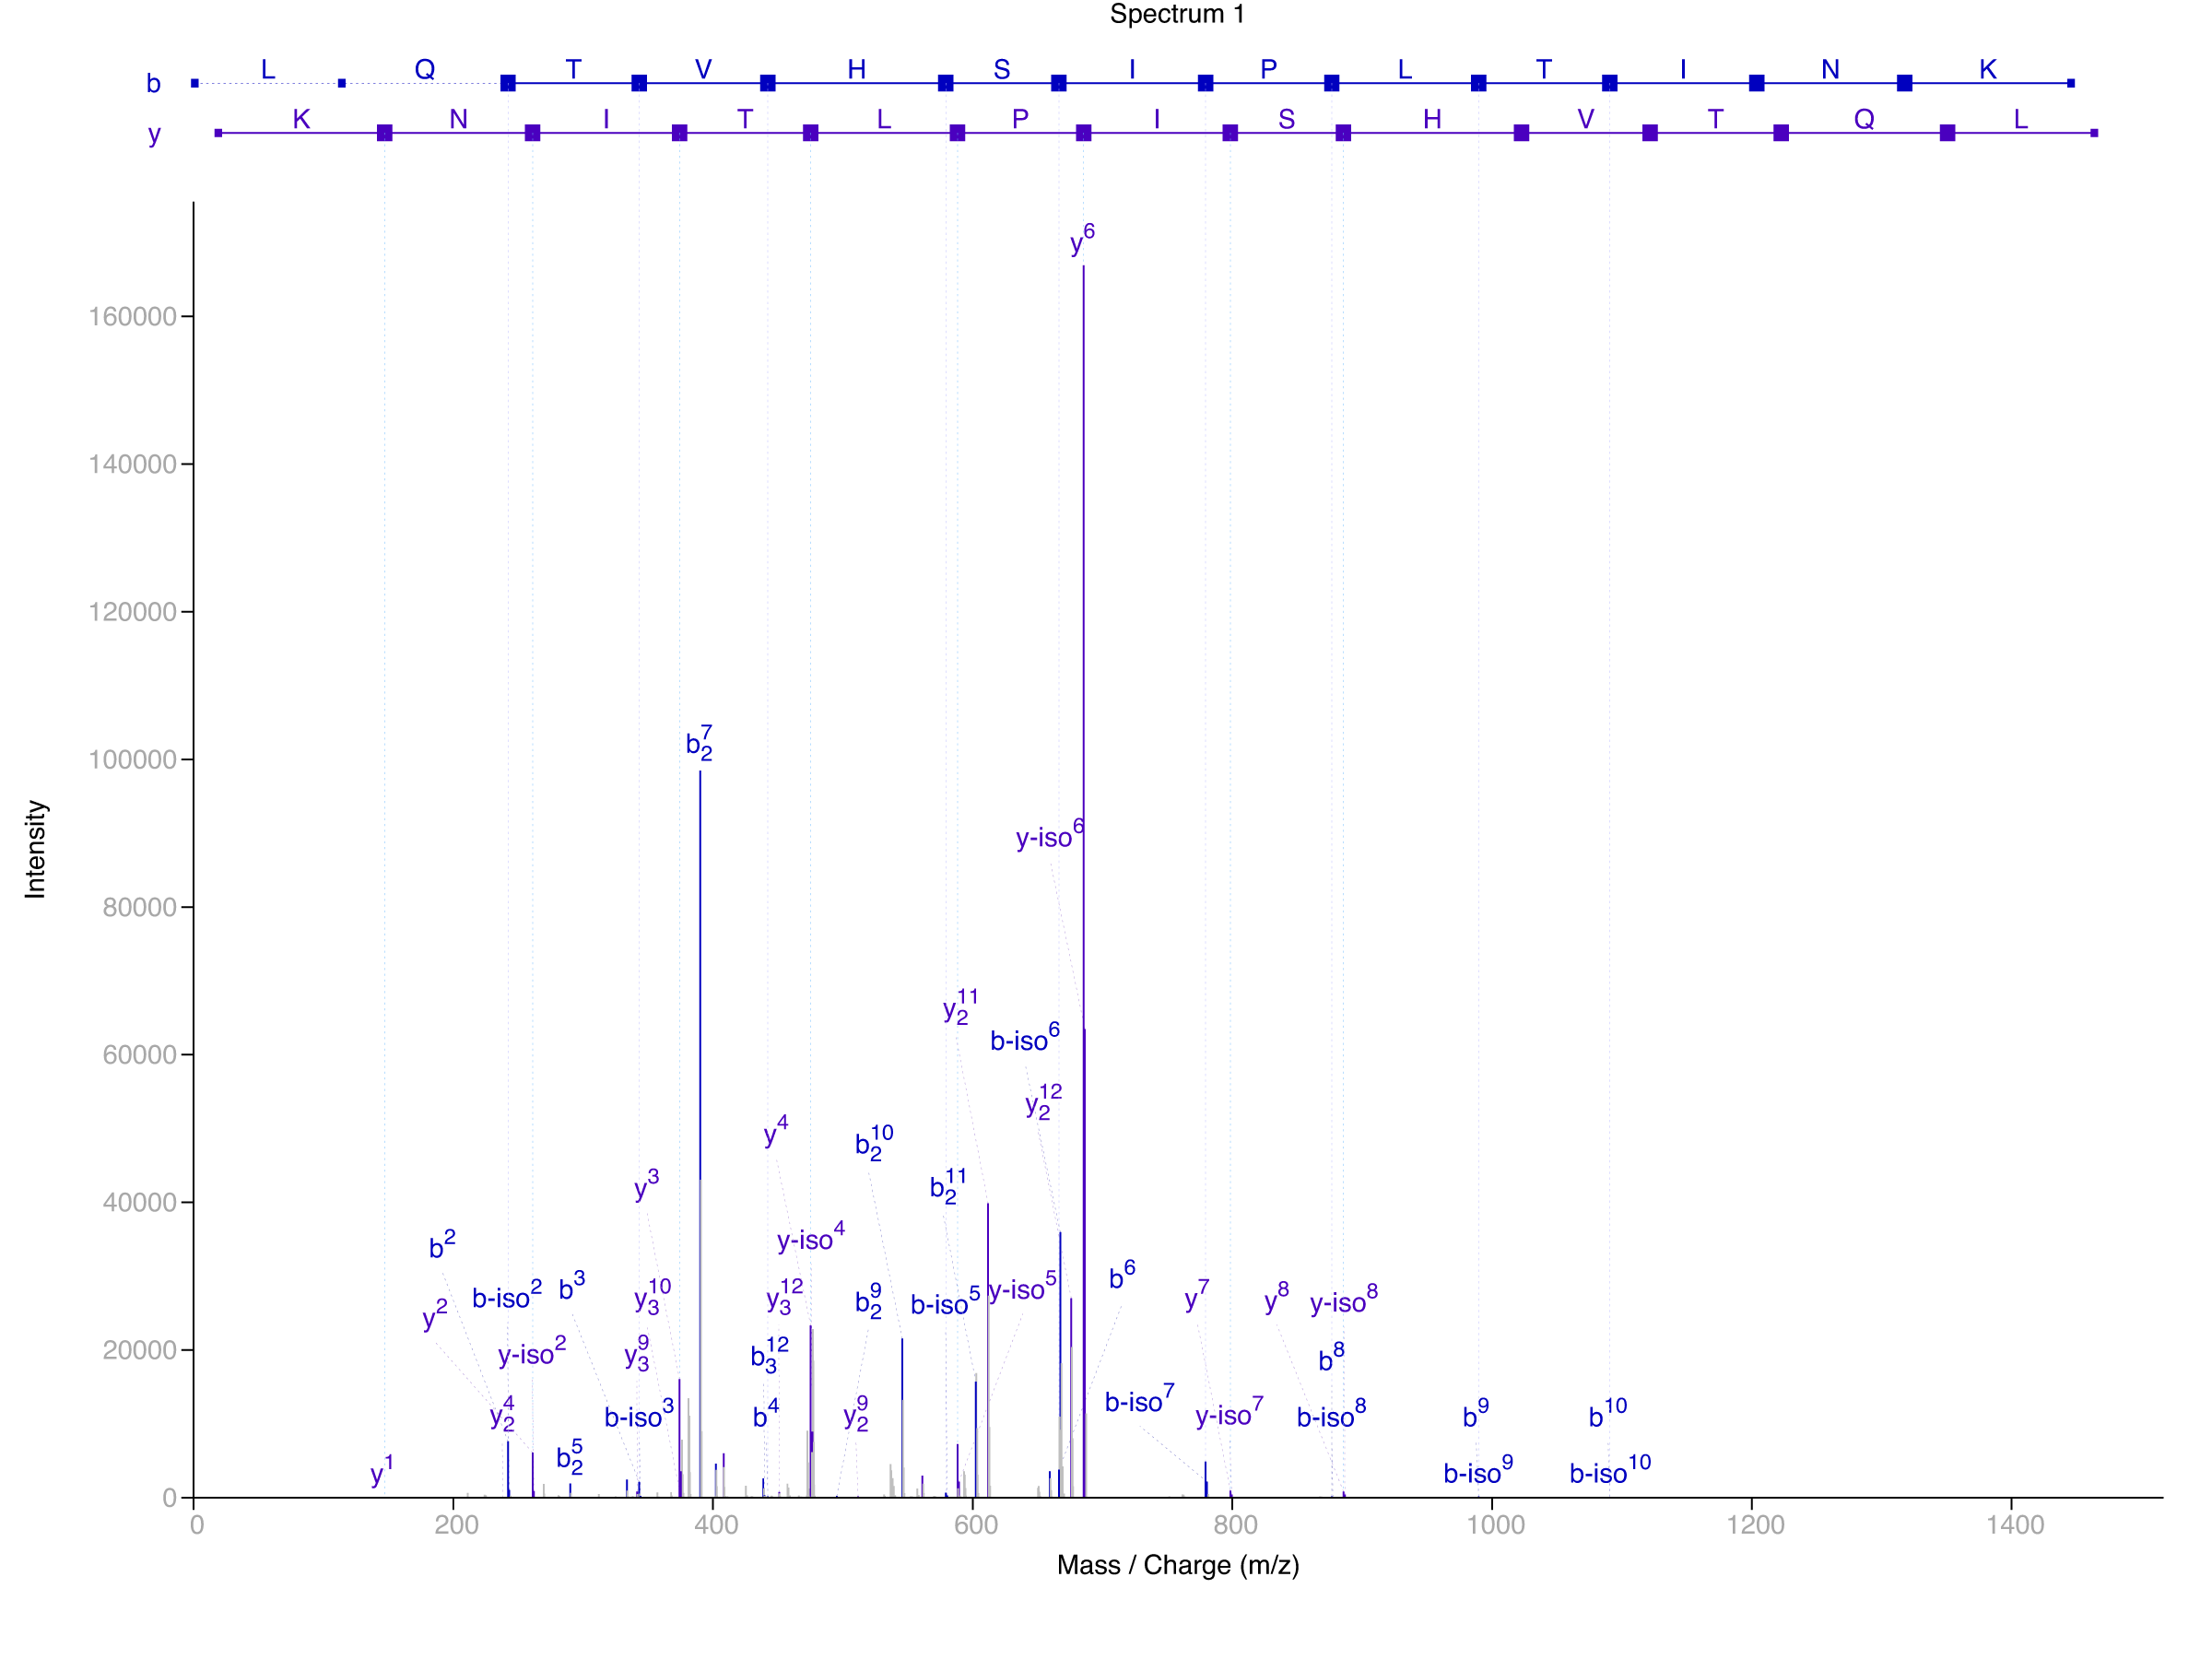
\includegraphics[scale=.37]{fig/synthetic/0055_LQ(T,-18)VHSIPLTINK_unmod.png}\\
b) 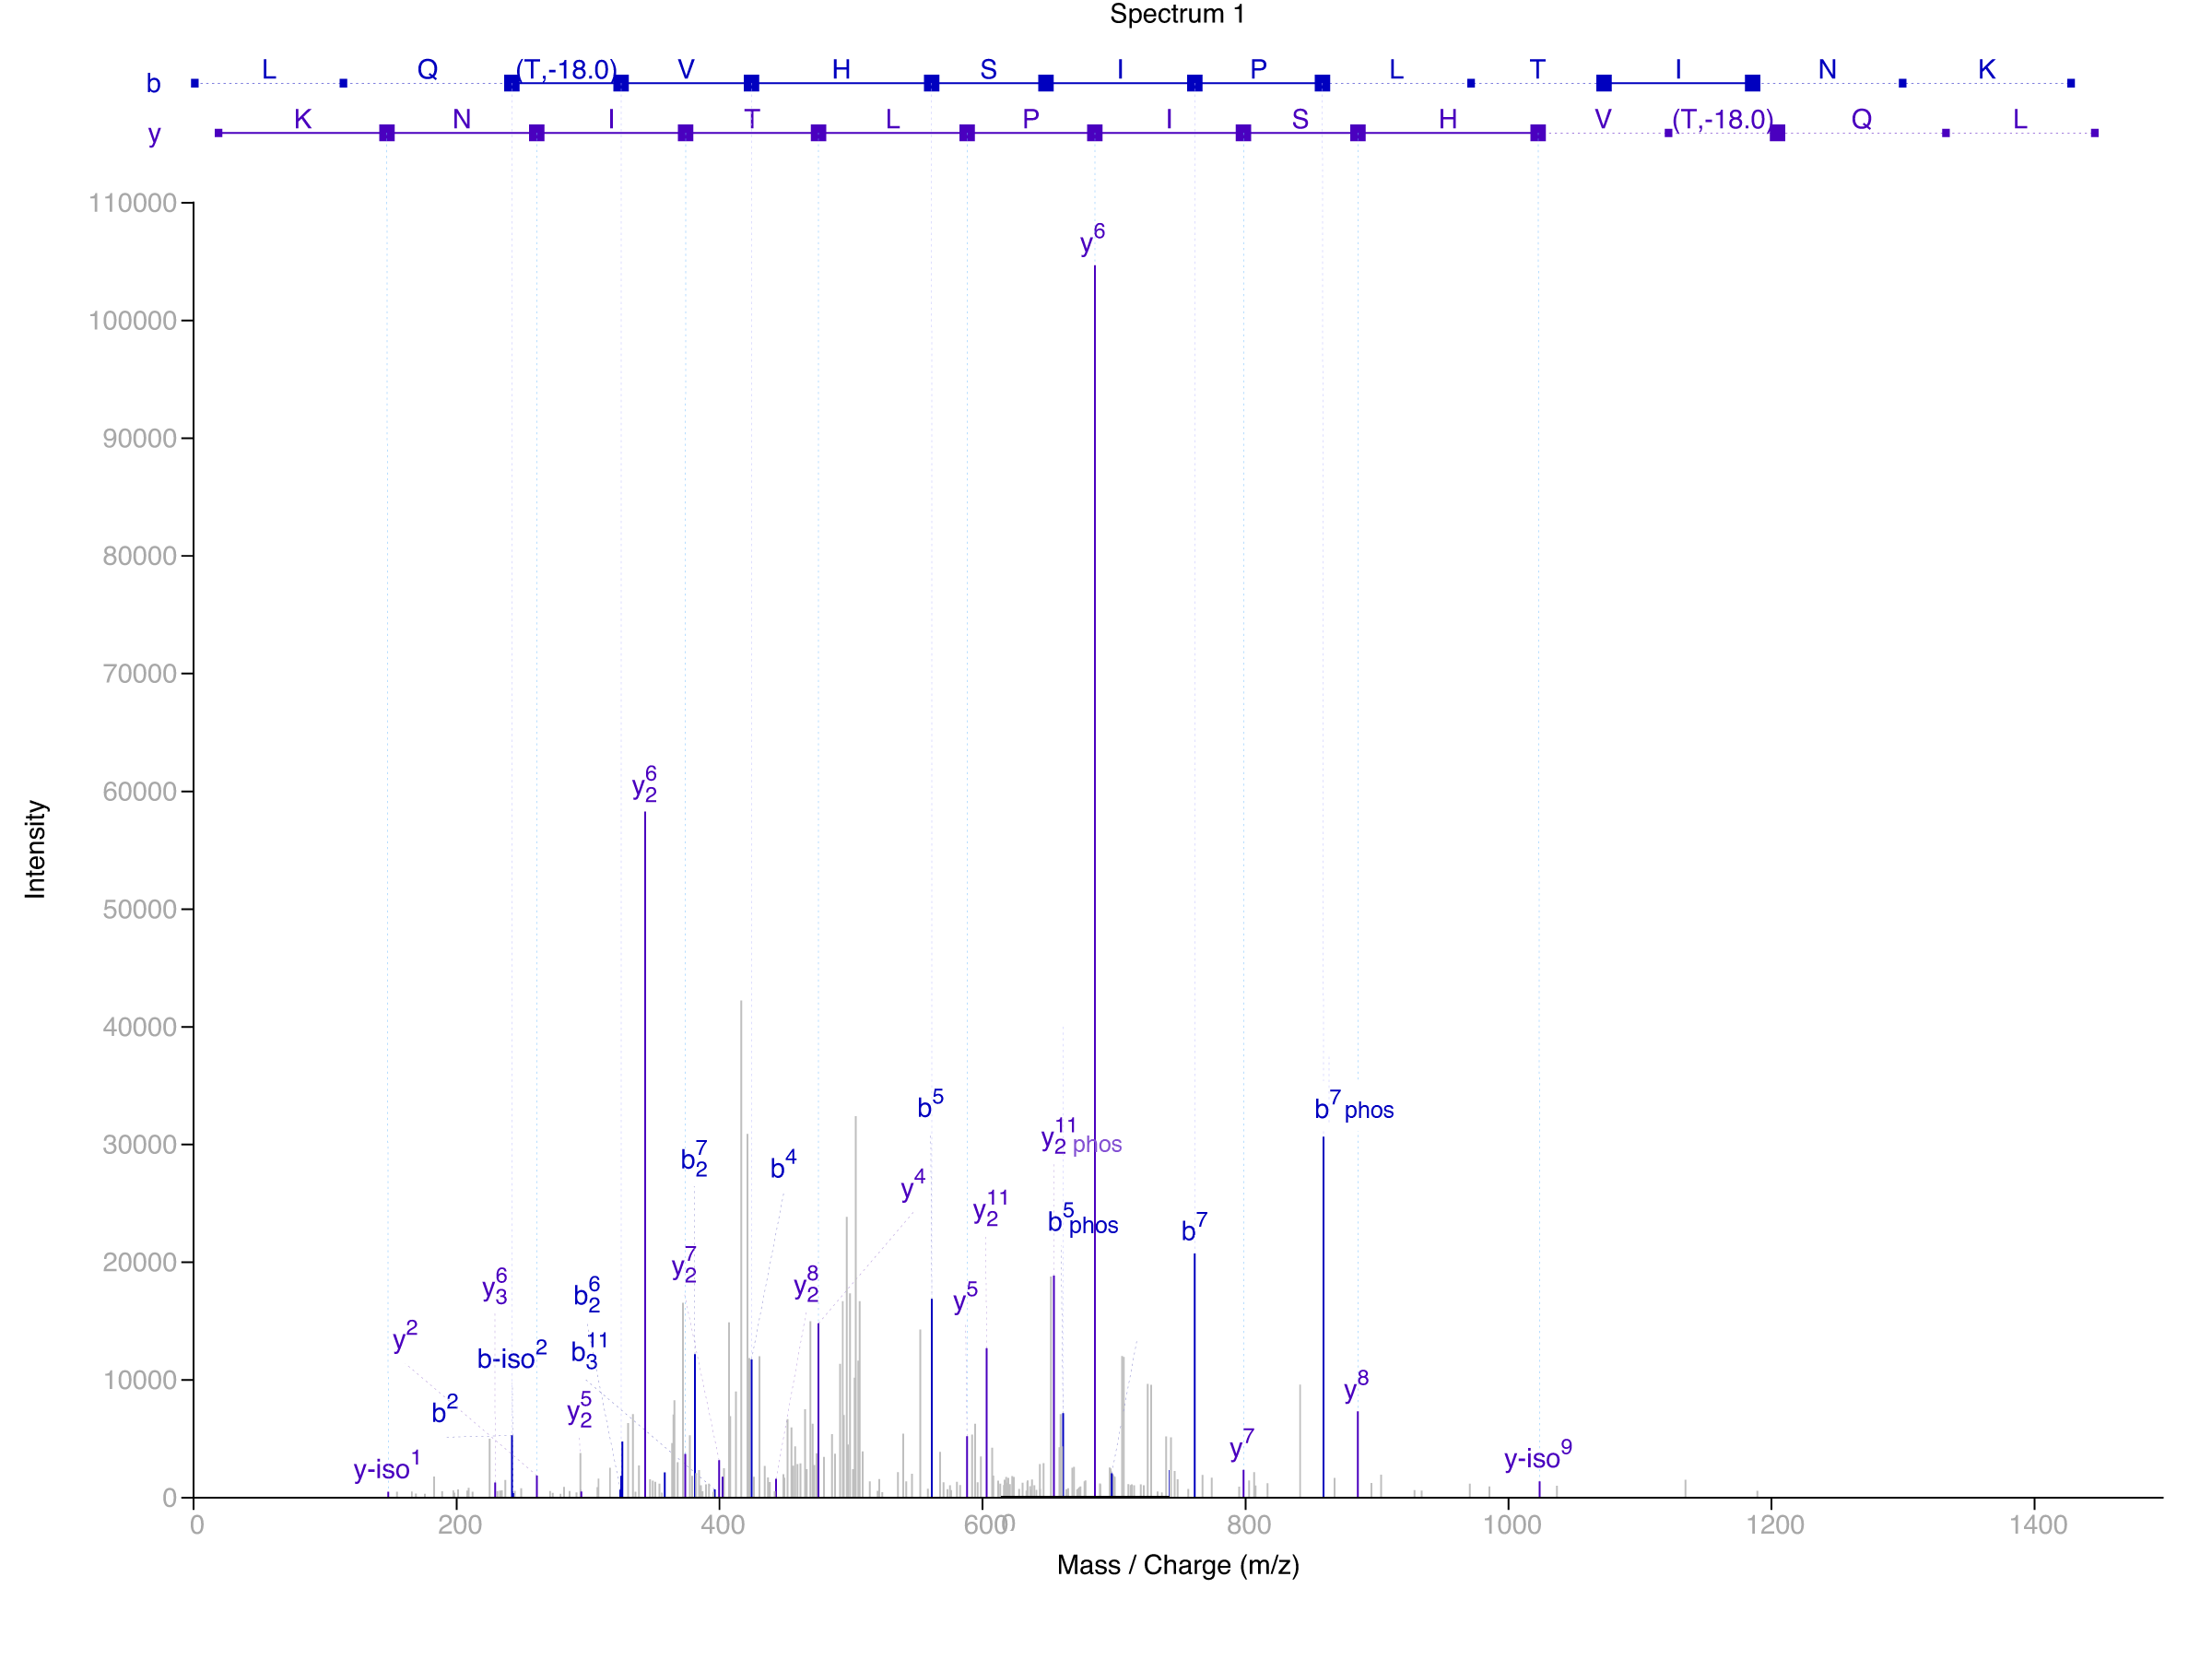
\includegraphics[scale=.37]{fig/synthetic/0055_LQ(T,-18)VHSIPLTINK_mod1.png}
c) 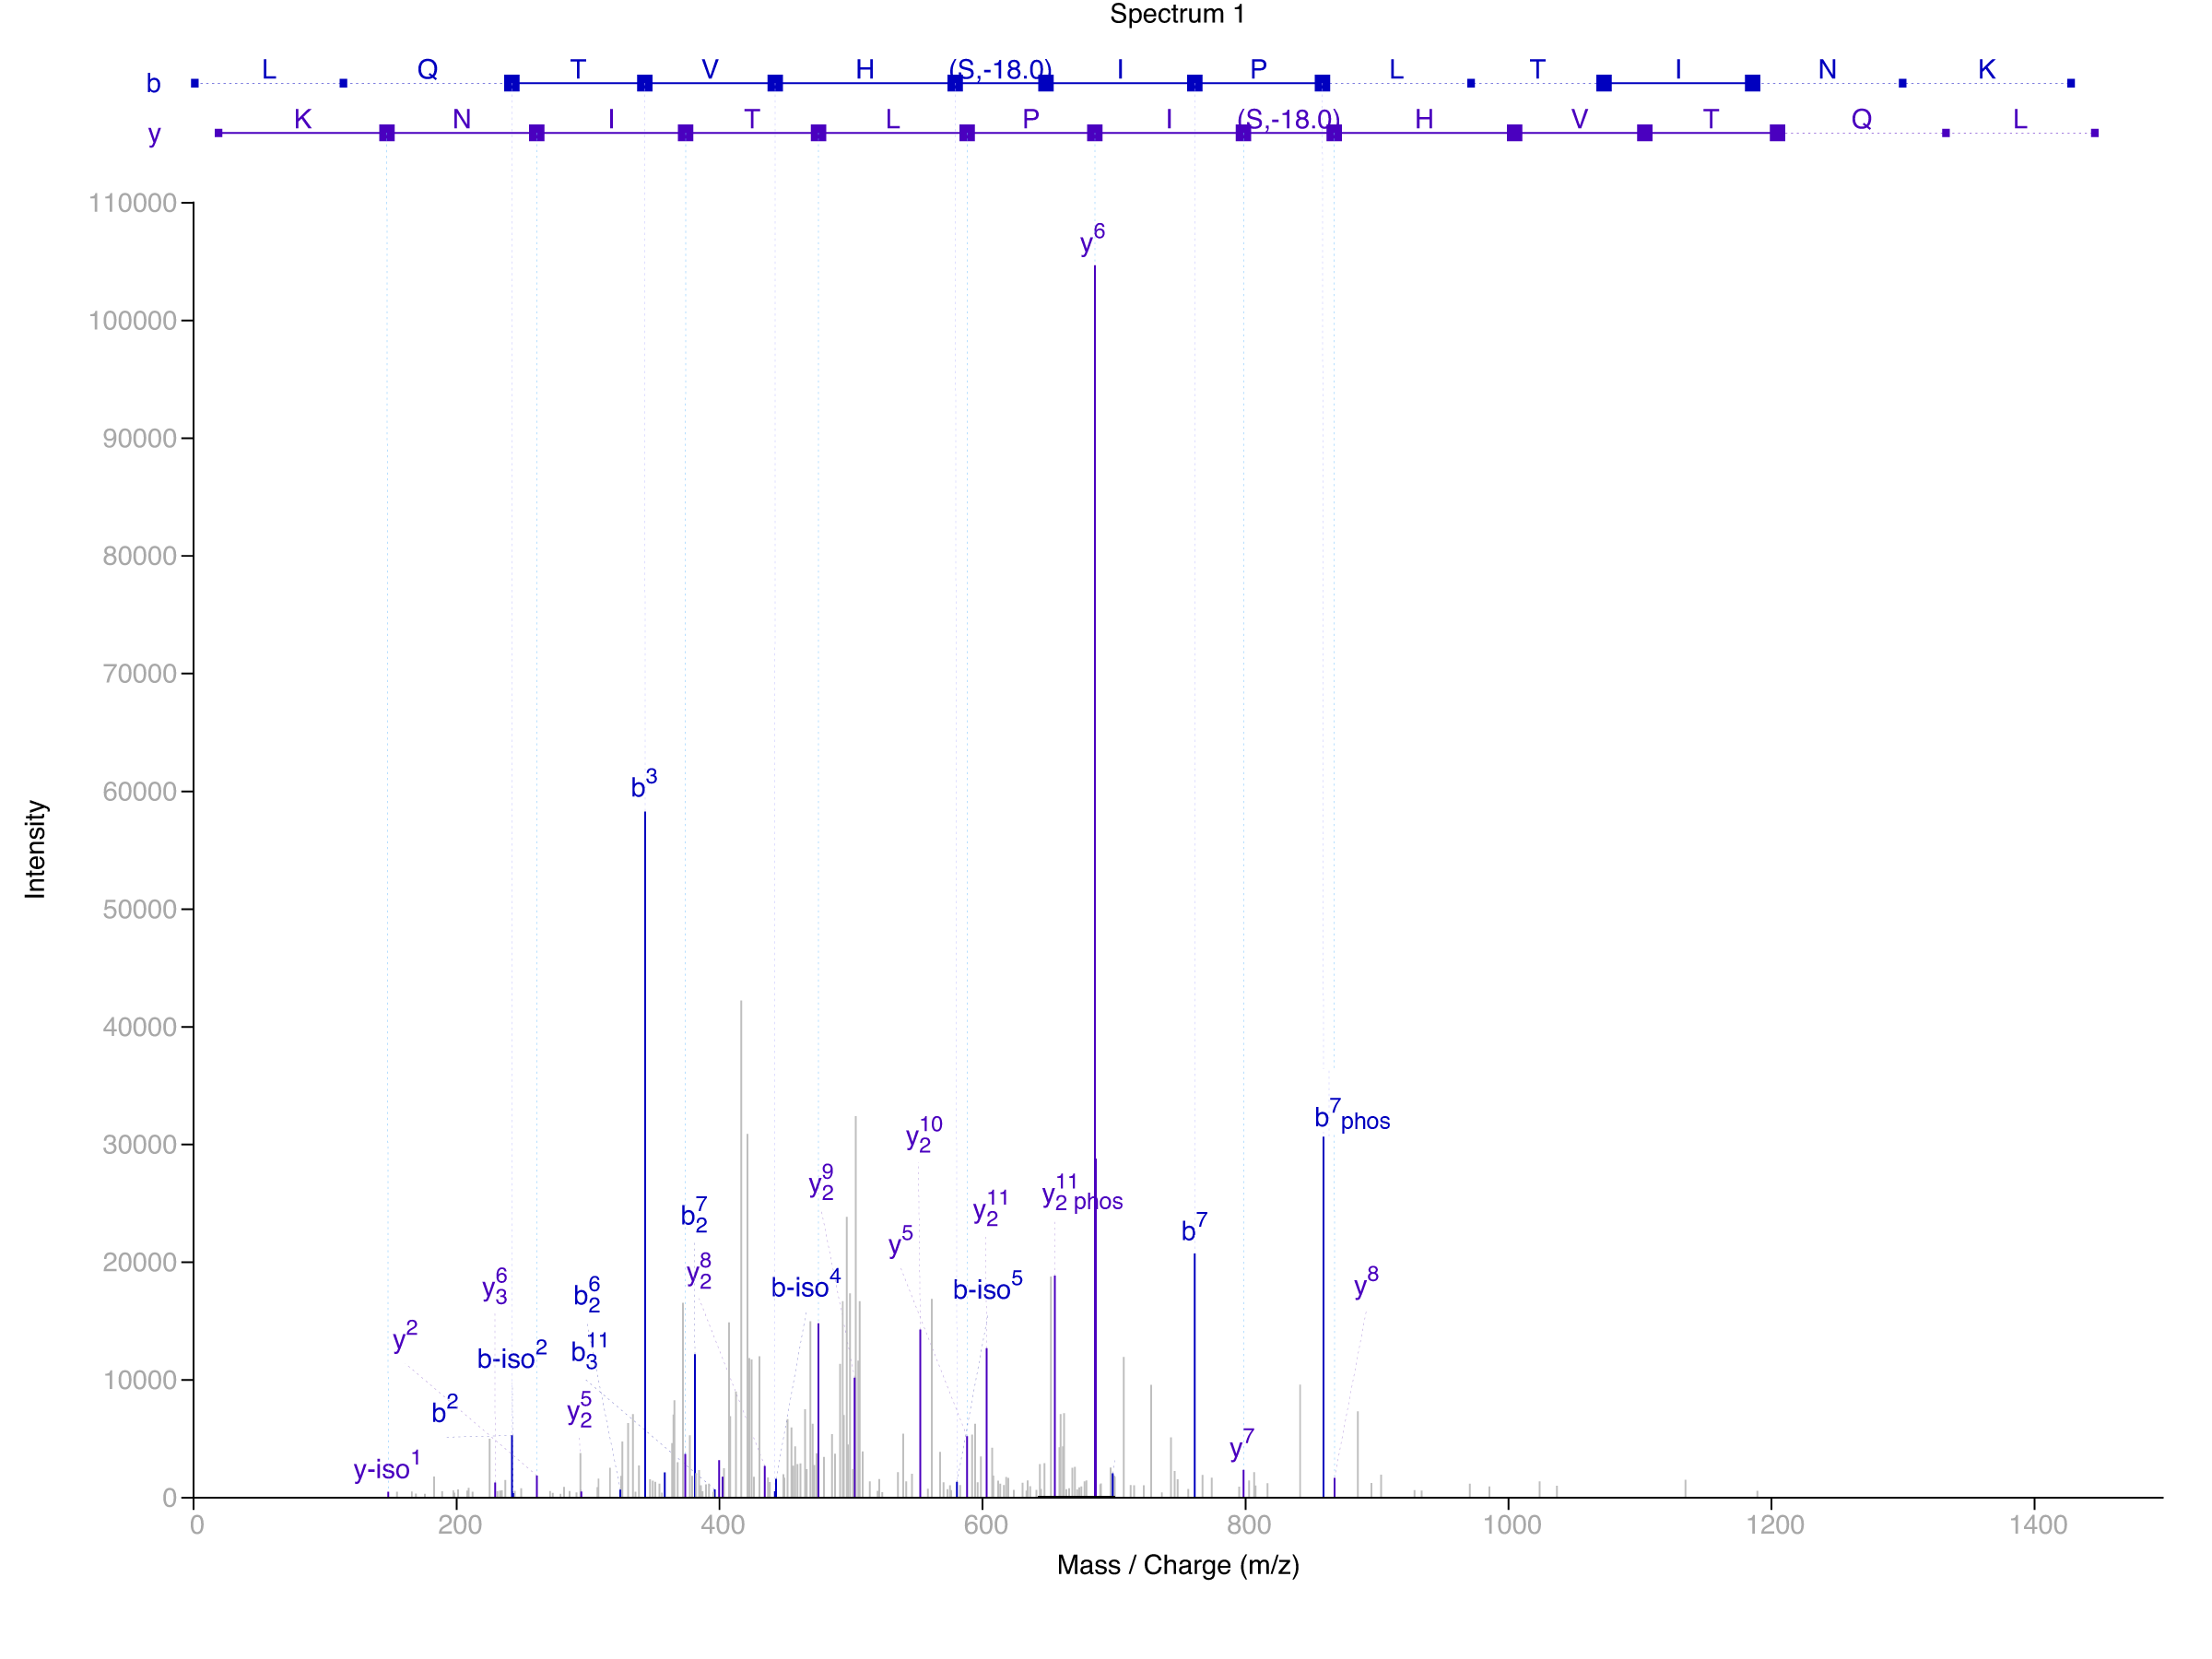
\includegraphics[scale=.37]{fig/synthetic/0055_LQ(T,-18)VHSIPLTINK_mod2.png}
\caption[Modification assignment comparison]{Comparison of unmodified and modified spectra with two possible modification assignments. Note that while phosphorylated fragments are labeled, they are not included in the LP score. a) Unmodified charge 3 spectrum used for LP b) Scan 975 from  ppeptidemix1\_CID\_Orbi.mgf with expected synthetic modification site c) Scan 975 from  ppeptidemix1\_CID\_Orbi.mgf with site assigned by LP}
\label{fig:charge3Incorrect}
\end{figure} 